%%%%%%%%%%%%%%%%%%%%%%%%%%%%%%%
%This is the article LaTeX template for RSC journals
%Copyright The Royal Society of Chemistry 2010
%%%%%%%%%%%%%%%%%%%%%%%%%%%%%%%


\documentclass[8.5pt,twoside,twocolumn]{article}
\oddsidemargin -1.2cm
\evensidemargin -1.2cm
\textwidth 18cm
\headheight 1.0in
\topmargin -3.5cm
\textheight 22cm
\usepackage[super,sort&compress,comma]{natbib} 
\usepackage[version=3]{mhchem}
\usepackage[utf8]{inputenc}
\usepackage{times,mathptmx}
% \usepackage{times}
% feel free not to use mathptmx if it causes difficulties
\usepackage{sectsty}
\usepackage{balance} 

\usepackage{graphicx} %eps figures can be used instead
\usepackage{lastpage}
\usepackage[format=plain,justification=raggedright,singlelinecheck=false,font=small,labelfont=bf,labelsep=space]{caption} 
\usepackage{fancyhdr}
\pagestyle{fancy}

\begin{document}

%\thispagestyle{plain}
%\fancypagestyle{plain}{
%\fancyhead[L]{
\includegraphics[height=8pt]{headers/LH}}
%\fancyhead[C]{\hspace{-1cm}
\includegraphics[height=20pt]{headers/CH}}
%\fancyhead[R]{
\includegraphics[height=10pt]{headers/RH}\vspace{-0.2cm}}
%\renewcommand{\headrulewidth}{1pt}}
%\renewcommand{\thefootnote}{\fnsymbol{footnote}}
%\renewcommand\footnoterule{\vspace*{1pt}% 
%\hrule width 3.4in height 0.4pt \vspace*{5pt}} 
%\setcounter{secnumdepth}{5}



\makeatletter 
\def\subsubsection{\@startsection{subsubsection}{3}{10pt}{-1.25ex plus -1ex minus -.1ex}{0ex plus 0ex}{\normalsize\bf}} 
\def\paragraph{\@startsection{paragraph}{4}{10pt}{-1.25ex plus -1ex minus -.1ex}{0ex plus 0ex}{\normalsize\textit}} 
\renewcommand\@biblabel[1]{#1}            
\renewcommand\@makefntext[1]% 
{\noindent\makebox[0pt][r]{\@thefnmark\,}#1}
\makeatother 
\renewcommand{\figurename}{\small{Fig.}~}
\sectionfont{\large}
\subsectionfont{\normalsize} 

%\fancyfoot{}
%\fancyfoot[LO,RE]{\vspace{-7pt}
\includegraphics[height=9pt]{headers/LF}}
%\fancyfoot[CO]{\vspace{-7.2pt}\hspace{12.2cm}
\includegraphics{headers/RF}}
%\fancyfoot[CE]{\vspace{-7.5pt}\hspace{-13.5cm}
\includegraphics{headers/RF}}
%\fancyfoot[RO]{\footnotesize{\sffamily{1--\pageref{LastPage} ~\textbar  \hspace{2pt}\thepage}}}
%\fancyfoot[LE]{\footnotesize{\sffamily{\thepage~\textbar\hspace{3.45cm} 1--\pageref{LastPage}}}}
\fancyhead{}
\renewcommand{\headrulewidth}{1pt} 
\renewcommand{\footrulewidth}{1pt}
\setlength{\arrayrulewidth}{1pt}
\setlength{\columnsep}{6.5mm}
\setlength\bibsep{1pt}

\twocolumn[
  \begin{@twocolumnfalse}
\noindent\LARGE{\textbf{Self-sustained carbon monoxide oxidation oscillations on size-selected platinum nanoparticles at atmospheric pressure$^\dag$}}
\vspace{0.6cm}

\noindent\large{\textbf{Robert Jensen\textit{$^{a}$}, Thomas Andersen\textit{$^{a}$}, Anders Nierhoff\textit{$^{a}$}, Thomas Pedersen\textit{$^{b}$}, Ole Hansen\textit{$^{b}$}, Søren Dahl\textit{$^{a}$} and Ib Chorkendorff\textit{$^{a}$}}}\vspace{0.5cm}
%Please note that \ast indicates the corresponding author(s) but no footnote text is required. 


%\noindent\textit{\small{\textbf{Received Xth XXXXXXXXXX 20XX, Accepted Xth XXXXXXXXX 20XX\newline
%First published on the web Xth XXXXXXXXXX 200X}}}

%\noindent \textbf{\small{DOI: 10.1039/b000000x}}
\vspace{0.6cm}
%Please do not change this text.

\noindent \normalsize{High-quality mass spectrometry data of the oscillatory behavior of CO oxidation on SiO$_2$ supported Pt-nanoparticles at atmospheric pressure has been acquired as a function of pressure, coverage, gas composition and nanoparticle size. The oscillations are self-sustained for several days at constant temperature, pressure and CO/O$_2$ ratio. The frequency of the oscillations is very well defined and increases over time. The oscillation frequency is furthermore strongly temperature dependent with increasing temperature resulting in increasing frequency. A plausible mechanism for the oscillations is proposed based on a oxidation/reduction cycle of the nanoparticles which change the rate of CO oxidation on the particles.}  %on an earlier model on Pd single crystals [Hendriksen \textit{et al., Nature Chemistry}, 2010, \textbf{9}, 730]}
\vspace{0.5cm}
 \end{@twocolumnfalse}
  ]


%\section{This is the section heading style}
\section{Introduction}
The experiments were performed in Si-based 20x15 mm $\mu$-reactors\cite{Henriksen2009}. The reactor consists of two inlets, a mixing zone allowing for diffusional mixing of reactants, an outlet, a reactor volume of $240\,$nL and a $5.4\,\mu$m wide capillary used for sniffing gases from the reactor volume. The reactor is sealed by anodic bonding of a pyrex lid to the Si reactor and is able to operate at a pressure range of 0-2.5\,bar. The reaction gases is supplied to the two inlets by flow controllers capable of controlling the gas flow from 0-10 mL/min. The capillary flow is fed into a quadropole mass-spectrometer (QMA) for analysis while any surplus of gas from the inlets are passed directly through to the outlet via a pressure controller allowing control of reactor pressure. The design makes sure that all gases exposed to the catalyst under investigation is measured by the QMA ensuring an extremely high sensitivity of the system. 

Before any measurements are performed the reactor is pumped by a turbopump to minimize contaminants in the system. When an evacuated reactor is mounted the base pressure of the mass spectrometer chamber is $\sim5\times10^{-9}\,$mbar and in operation at $1\,$bar in the reactor volume the pressure is $\sim5\times10^{-7}\,$mbar in the QMA chamber. 

The reactor is heated by joule heating of a Pt strip evaporated on the backside of the reactor volume. The introduction of two additional contacts on the backside of the reactor allows for 4 wire measurements of the resistance of the Pt strip using it as a RTD for temperature measurement of the reactor. An external thermocouple acts as room-temperature calibration of the RTD as well as sanity check of the RTD measurement during operation.

The gas handling including flow and pressured controllers and the mass spectrometer is fully automized allowing for measurements of several days without human intervention allowing for self-consistent measurements of many samples.

\subsection{Pt nanoparticle deposition}
Pt nanoparticles were deposited in the reactor using a gas-aggregation source (Mantis Deposition Ltd., Nanogen 50). Pt clusters were formed by gas-phase condensation of Pt atoms produced by impinging argon ions on a 99.99\% Pt target in a magnetron sputter source. After condensation the ionised fraction (60-80\%) of the clusters were size-selected by a quadropole mass selection filter according to their mass-to-charge ratio. Using this setup Pt nanoparticles with diameters in the range of 2--16\,nm can be produced \cite{Nielsen2010,Nielsen2009}. The size-selected nanoparticles were after size-selection soft-landed in the reactor volume of the microreactor. The coverage was kept at approximately 0.1\% geometric coverage determined by measuring the current on the reactor during deposition. After deposition the reactors were anodicly cold-bonded \cite{Vesborg2010} to a pyrex lid to avoid sintering of the nanoparticles while bonding.


\begin{figure}[h]
\centering
  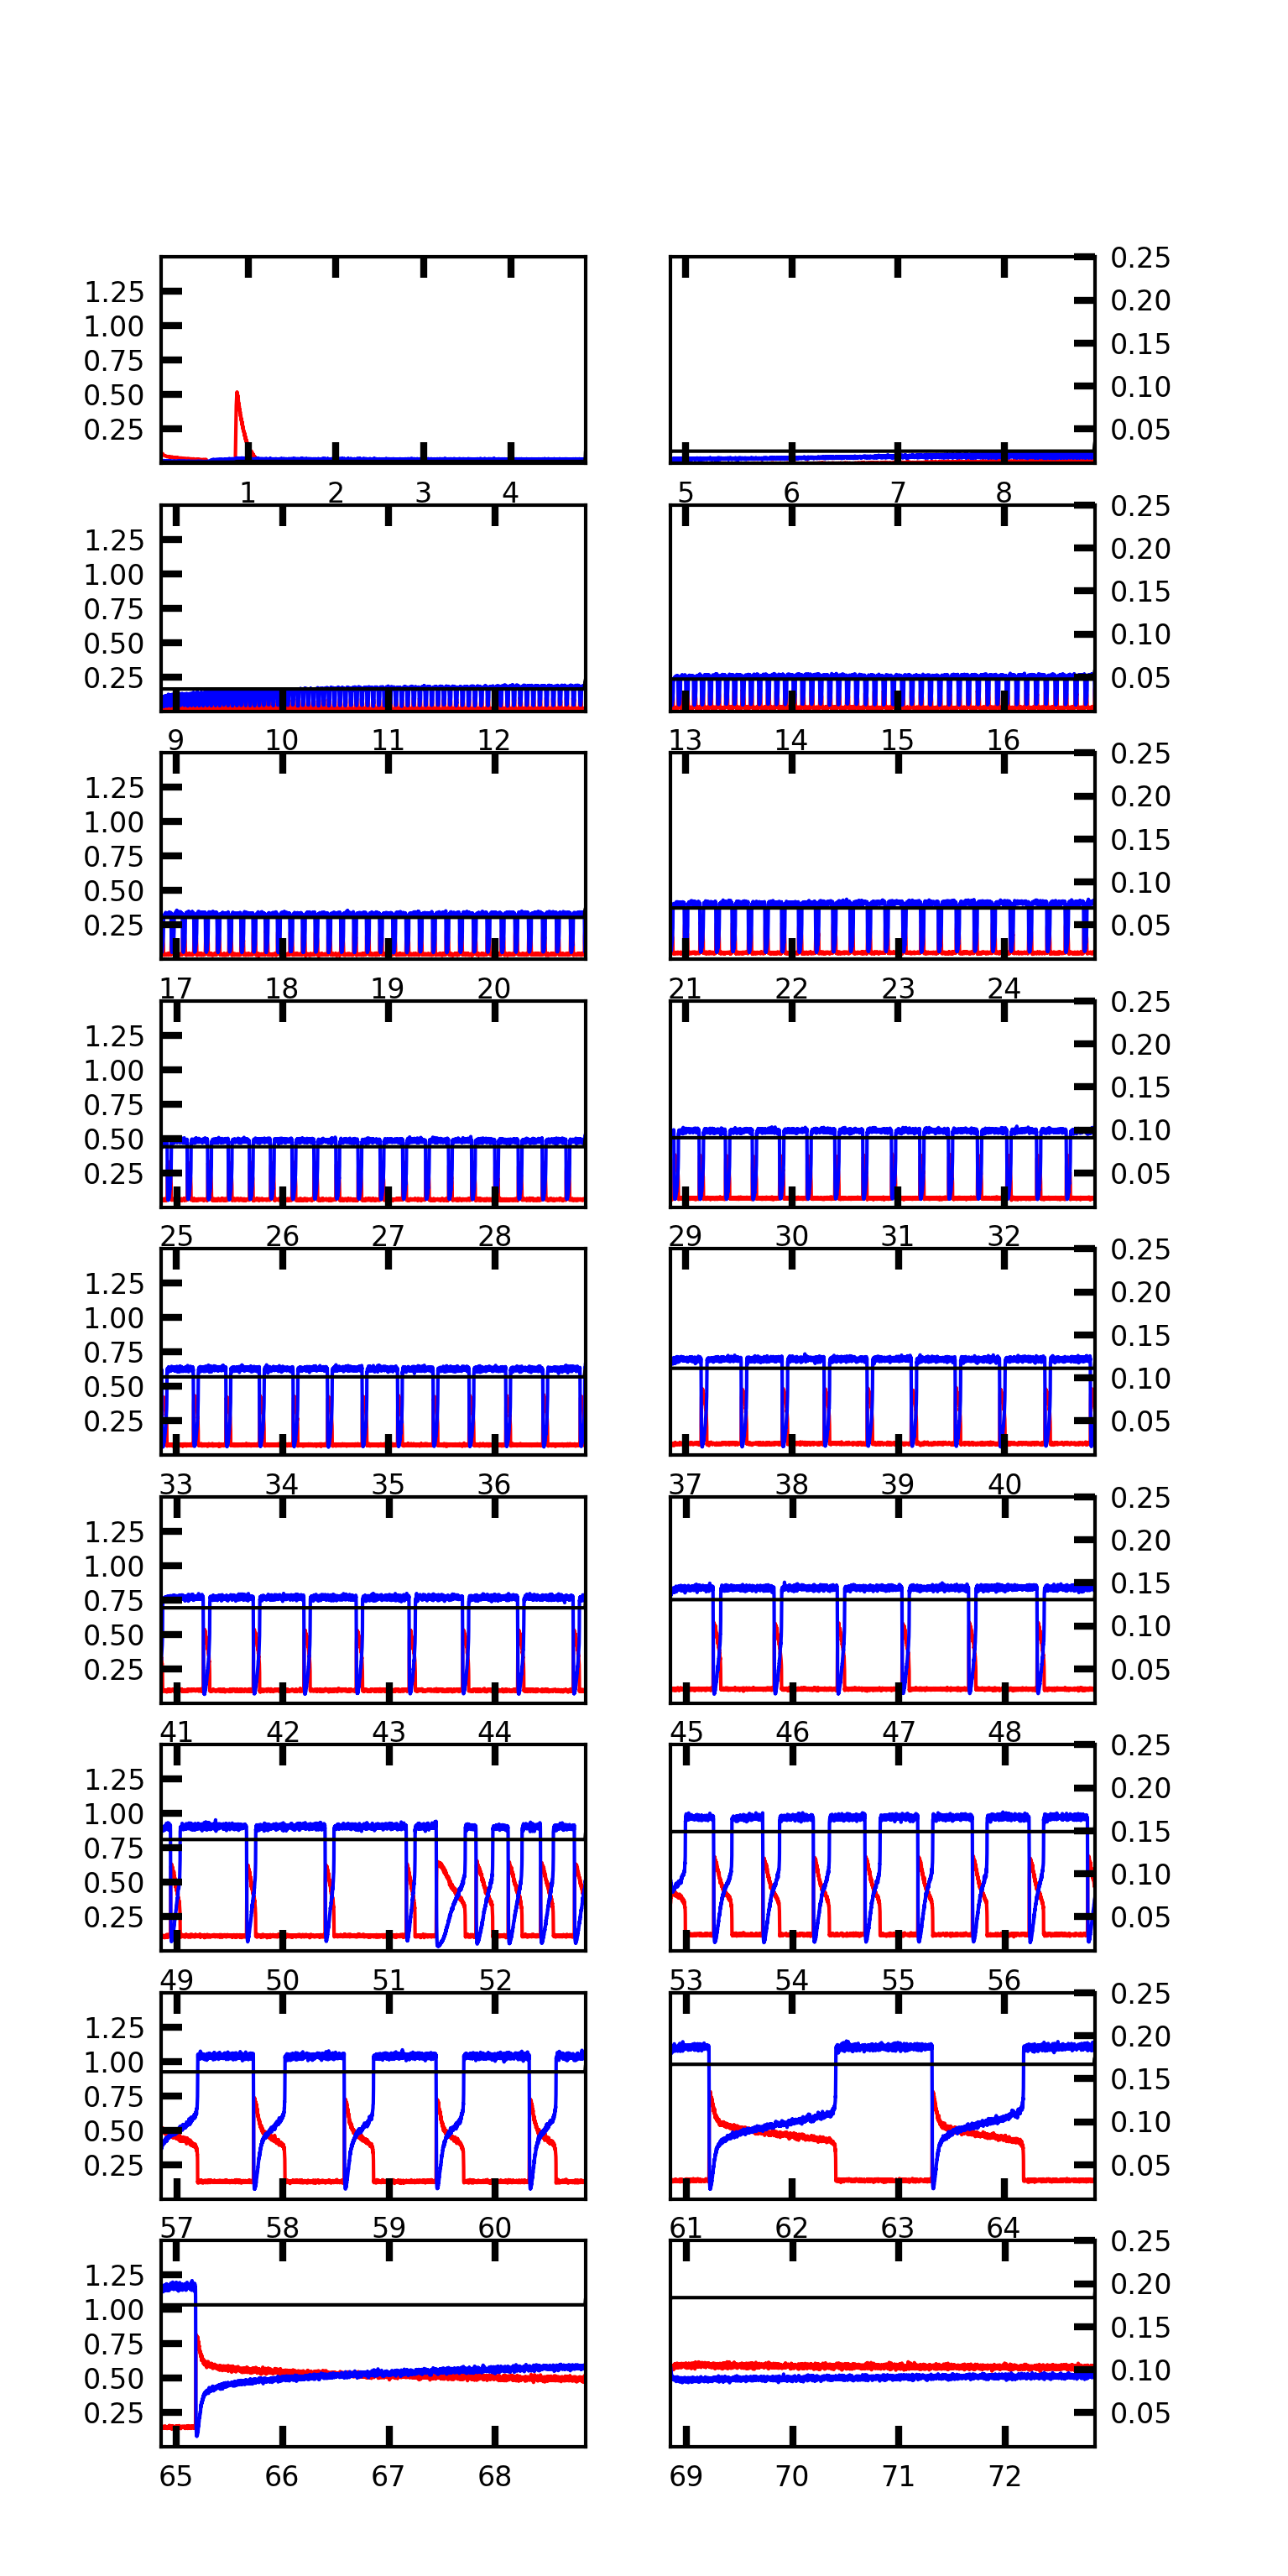
\includegraphics[width=13cm]{oscillations_gas_dependence_supplemental.png}
  \caption{Complete series of oscillating sample. For every frame the CO-concentration is increased.}
  \label{fgr:gas_dependence}
\end{figure}


\begin{figure}[h]
  \centering
  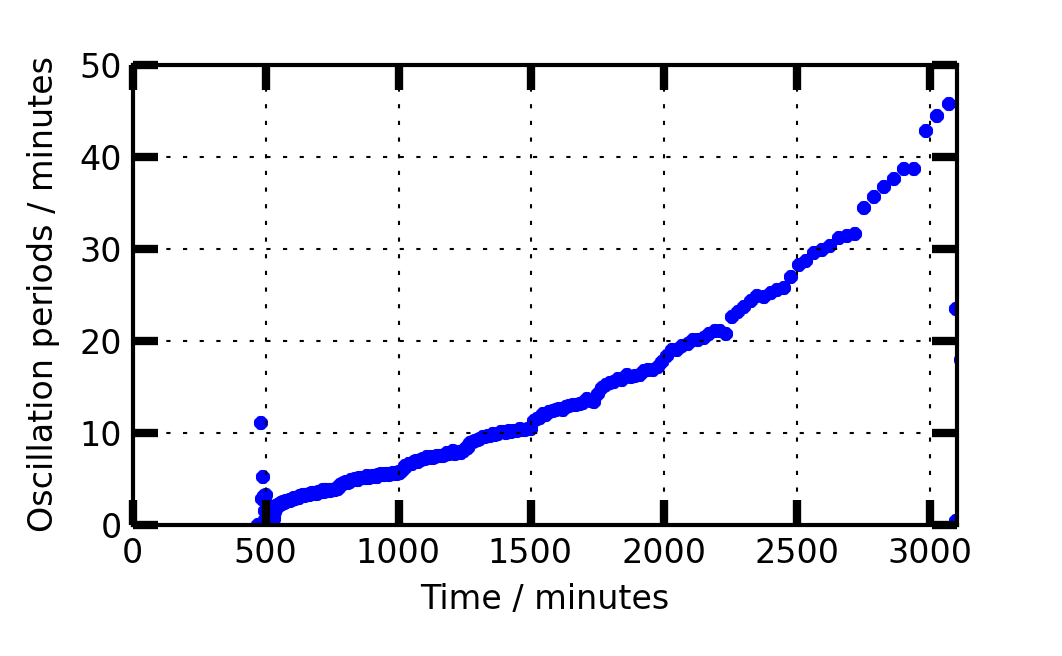
\includegraphics[width=9cm]{oscillations_gas_dependence_summary_supplemental.png}
  \caption{Summary of the gas-dependence. The overall trend of increasing oscillation period is now supporimposed by small discontinous stpes when the CO concentration is increased.}
  \label{fgr:gas_dependence_summary}
\end{figure}

\begin{figure}[h]
\centering
  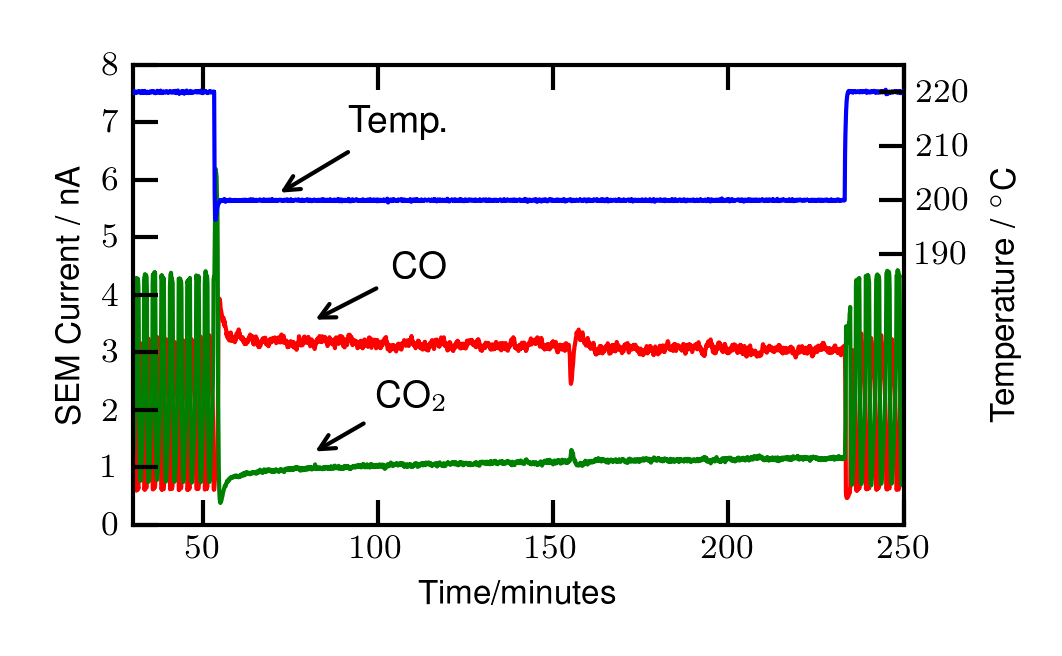
\includegraphics[width=9cm]{temperature_dependence_supplemental.png}
  \caption{Another example of the very pronounced temperature dependence. In this case the oscillations are switched on and off by a step of 20$^\circ$C}
  \label{fgr:temperature_dependence_supplemental}
\end{figure}


\begin{figure}[h]
\centering
  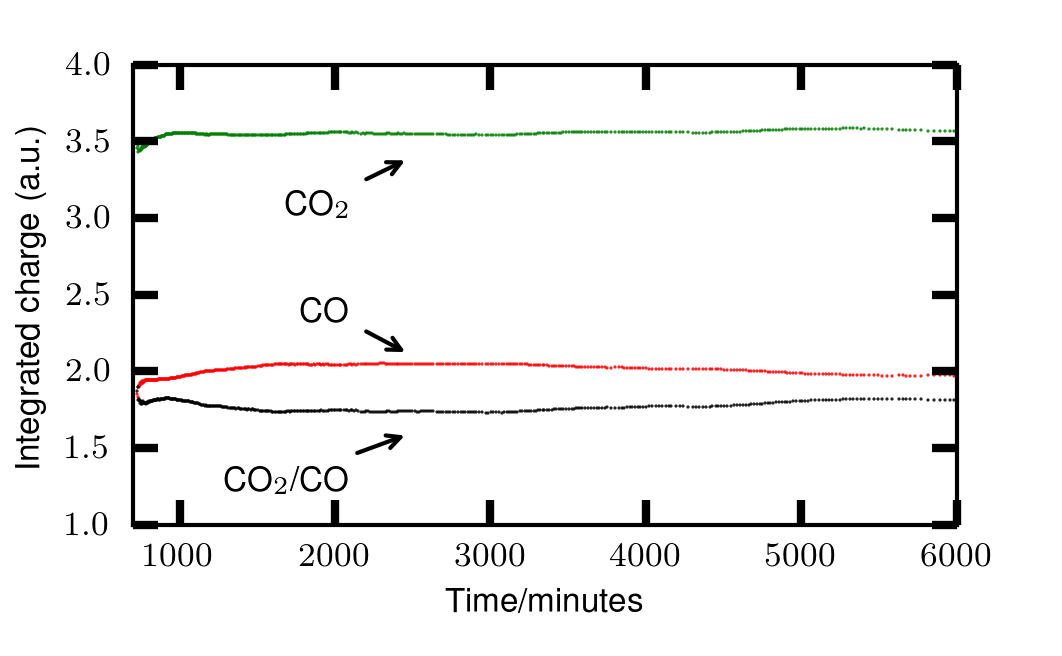
\includegraphics[width=9cm]{duty_cycles_long_measurement_supplemental.png}
  \caption{A plot of the duty-cycle of the sample duing the 4-day long experiment}
  \label{fgr:temperature_dependence_supplemental}
\end{figure}



\footnotesize{
\bibliography{literature} %your .bib file
\bibliographystyle{rsc} %the RSC's .bst file
}

\end{document}
